\documentclass[14pt]{extbook}
\usepackage{multicol, enumerate, enumitem, hyperref, color, soul, setspace, parskip, fancyhdr} %General Packages
\usepackage{amssymb, amsthm, amsmath, latexsym, units, mathtools} %Math Packages
\everymath{\displaystyle} %All math in Display Style
% Packages with additional options
\usepackage[headsep=0.5cm,headheight=12pt, left=1 in,right= 1 in,top= 1 in,bottom= 1 in]{geometry}
\usepackage[usenames,dvipsnames]{xcolor}
\usepackage{dashrule}  % Package to use the command below to create lines between items
\newcommand{\litem}[1]{\item#1\hspace*{-1cm}\rule{\textwidth}{0.4pt}}
\pagestyle{fancy}
\lhead{Progress Quiz 8}
\chead{}
\rhead{Version A}
\lfoot{5493-4176}
\cfoot{}
\rfoot{Summer C 2021}
\begin{document}

\begin{enumerate}
\litem{
Construct the lowest-degree polynomial given the zeros below. Then, choose the intervals that contain the coefficients of the polynomial in the form $ax^3+bx^2+cx+d$.\[ \frac{-4}{3}, \frac{4}{5}, \text{ and } \frac{6}{5} \]\begin{enumerate}[label=\Alph*.]
\item \( a \in [70, 77], b \in [-53, -41], c \in [-130, -119], \text{ and } d \in [86, 98] \)
\item \( a \in [70, 77], b \in [50, 55], c \in [-130, -119], \text{ and } d \in [-100, -88] \)
\item \( a \in [70, 77], b \in [-53, -41], c \in [-130, -119], \text{ and } d \in [-100, -88] \)
\item \( a \in [70, 77], b \in [-251, -249], c \in [271, 273], \text{ and } d \in [-100, -88] \)
\item \( a \in [70, 77], b \in [-131, -126], c \in [-33, -27], \text{ and } d \in [86, 98] \)

\end{enumerate} }
\litem{
Describe the end behavior of the polynomial below.\[ f(x) = 5(x - 7)^{4}(x + 7)^{5}(x - 4)^{3}(x + 4)^{3} \]\begin{enumerate}[label=\Alph*.]
\begin{multicols}{2}\item 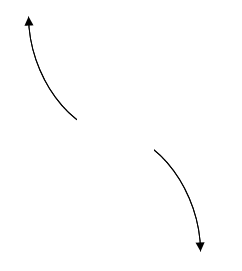
\includegraphics[width = 0.3\textwidth]{../Figures/polyEndBehaviorCopyAA.png}\item 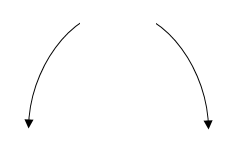
\includegraphics[width = 0.3\textwidth]{../Figures/polyEndBehaviorCopyBA.png}\item 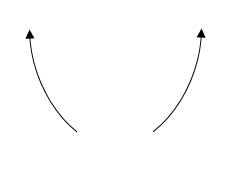
\includegraphics[width = 0.3\textwidth]{../Figures/polyEndBehaviorCopyCA.png}\item 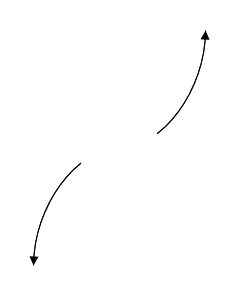
\includegraphics[width = 0.3\textwidth]{../Figures/polyEndBehaviorCopyDA.png}\end{multicols}\item None of the above.
\end{enumerate} }
\litem{
Construct the lowest-degree polynomial given the zeros below. Then, choose the intervals that contain the coefficients of the polynomial in the form $x^3+bx^2+cx+d$.\[ -2 + 4 i \text{ and } 1 \]\begin{enumerate}[label=\Alph*.]
\item \( b \in [0.7, 1.4], c \in [-6, -3], \text{ and } d \in [2, 11] \)
\item \( b \in [0.7, 1.4], c \in [-1, 5], \text{ and } d \in [-9, 0] \)
\item \( b \in [-6.9, -1.6], c \in [14, 23], \text{ and } d \in [13, 26] \)
\item \( b \in [1.6, 6.2], c \in [14, 23], \text{ and } d \in [-25, -14] \)
\item \( \text{None of the above.} \)

\end{enumerate} }
\litem{
Describe the end behavior of the polynomial below.\[ f(x) = -4(x - 4)^{5}(x + 4)^{10}(x + 6)^{3}(x - 6)^{5} \]\begin{enumerate}[label=\Alph*.]
\begin{multicols}{2}\item 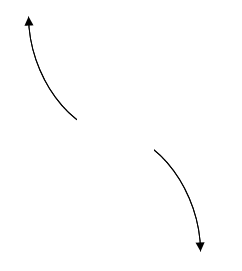
\includegraphics[width = 0.3\textwidth]{../Figures/polyEndBehaviorAA.png}\item 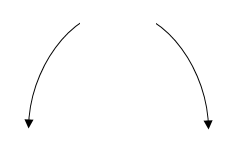
\includegraphics[width = 0.3\textwidth]{../Figures/polyEndBehaviorBA.png}\item 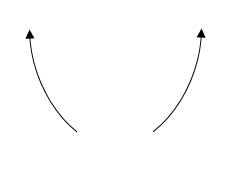
\includegraphics[width = 0.3\textwidth]{../Figures/polyEndBehaviorCA.png}\item 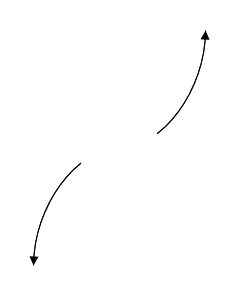
\includegraphics[width = 0.3\textwidth]{../Figures/polyEndBehaviorDA.png}\end{multicols}\item None of the above.
\end{enumerate} }
\litem{
Which of the following equations \textit{could} be of the graph presented below?
\begin{center}
    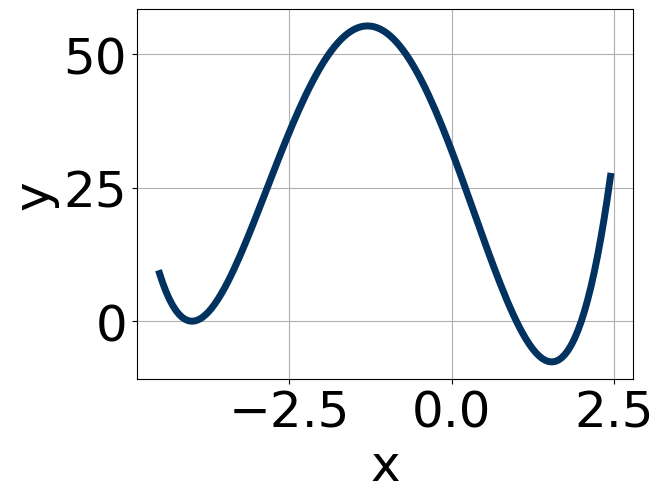
\includegraphics[width=0.5\textwidth]{../Figures/polyGraphToFunctionCopyA.png}
\end{center}
\begin{enumerate}[label=\Alph*.]
\item \( 10(x + 4)^{6} (x - 1)^{11} (x - 2)^{5} \)
\item \( 10(x + 4)^{8} (x - 1)^{10} (x - 2)^{5} \)
\item \( -12(x + 4)^{4} (x - 1)^{5} (x - 2)^{8} \)
\item \( -6(x + 4)^{10} (x - 1)^{11} (x - 2)^{11} \)
\item \( 17(x + 4)^{7} (x - 1)^{10} (x - 2)^{5} \)

\end{enumerate} }
\litem{
Describe the zero behavior of the zero $x = -5$ of the polynomial below.\[ f(x) = -9(x - 5)^{2}(x + 5)^{7}(x + 7)^{8}(x - 7)^{10} \]\begin{enumerate}[label=\Alph*.]
\begin{multicols}{2}\item 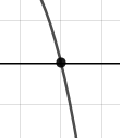
\includegraphics[width = 0.3\textwidth]{../Figures/polyZeroBehaviorAA.png}\item 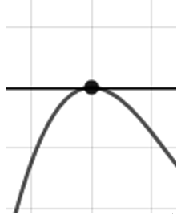
\includegraphics[width = 0.3\textwidth]{../Figures/polyZeroBehaviorBA.png}\item 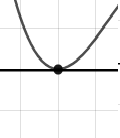
\includegraphics[width = 0.3\textwidth]{../Figures/polyZeroBehaviorCA.png}\item 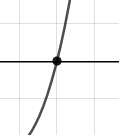
\includegraphics[width = 0.3\textwidth]{../Figures/polyZeroBehaviorDA.png}\end{multicols}\item None of the above.
\end{enumerate} }
\litem{
Construct the lowest-degree polynomial given the zeros below. Then, choose the intervals that contain the coefficients of the polynomial in the form $x^3+bx^2+cx+d$.\[ -2 - 3 i \text{ and } 2 \]\begin{enumerate}[label=\Alph*.]
\item \( b \in [-2.71, -1.5], c \in [3.3, 9.2], \text{ and } d \in [22.8, 26.7] \)
\item \( b \in [1.42, 2.12], c \in [3.3, 9.2], \text{ and } d \in [-26.6, -24.8] \)
\item \( b \in [0.14, 1.15], c \in [0.2, 1.1], \text{ and } d \in [-7.3, -4.4] \)
\item \( b \in [0.14, 1.15], c \in [-3.6, 0.6], \text{ and } d \in [-4.4, -1.3] \)
\item \( \text{None of the above.} \)

\end{enumerate} }
\litem{
Construct the lowest-degree polynomial given the zeros below. Then, choose the intervals that contain the coefficients of the polynomial in the form $ax^3+bx^2+cx+d$.\[ \frac{-1}{4}, 7, \text{ and } \frac{7}{5} \]\begin{enumerate}[label=\Alph*.]
\item \( a \in [18, 22], b \in [-170, -159], c \in [152, 163], \text{ and } d \in [42, 51] \)
\item \( a \in [18, 22], b \in [106, 113], c \in [-227, -221], \text{ and } d \in [42, 51] \)
\item \( a \in [18, 22], b \in [-178, -171], c \in [231, 239], \text{ and } d \in [-53, -47] \)
\item \( a \in [18, 22], b \in [159, 164], c \in [152, 163], \text{ and } d \in [-53, -47] \)
\item \( a \in [18, 22], b \in [-170, -159], c \in [152, 163], \text{ and } d \in [-53, -47] \)

\end{enumerate} }
\litem{
Which of the following equations \textit{could} be of the graph presented below?
\begin{center}
    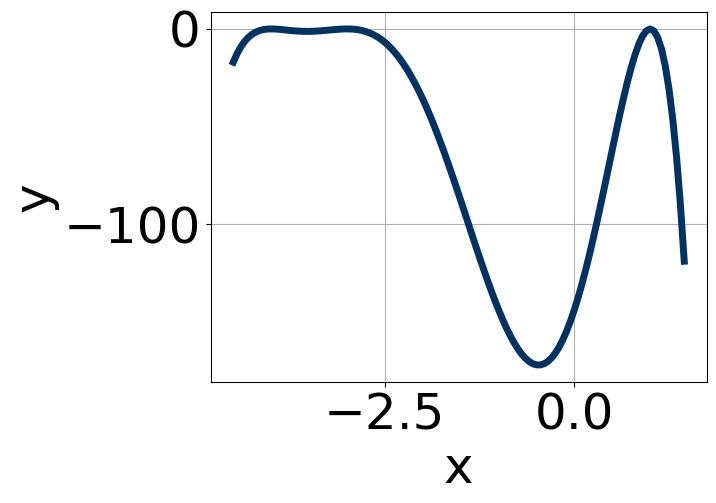
\includegraphics[width=0.5\textwidth]{../Figures/polyGraphToFunctionA.png}
\end{center}
\begin{enumerate}[label=\Alph*.]
\item \( -20(x + 4)^{10} (x + 3)^{5} (x - 1)^{7} \)
\item \( 9(x + 4)^{8} (x + 3)^{8} (x - 1)^{9} \)
\item \( 10(x + 4)^{4} (x + 3)^{10} (x - 1)^{6} \)
\item \( -3(x + 4)^{6} (x + 3)^{6} (x - 1)^{8} \)
\item \( -16(x + 4)^{6} (x + 3)^{4} (x - 1)^{5} \)

\end{enumerate} }
\litem{
Describe the zero behavior of the zero $x = 7$ of the polynomial below.\[ f(x) = -7(x + 7)^{5}(x - 7)^{10}(x - 4)^{4}(x + 4)^{7} \]\begin{enumerate}[label=\Alph*.]
\begin{multicols}{2}\item 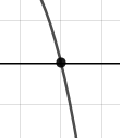
\includegraphics[width = 0.3\textwidth]{../Figures/polyZeroBehaviorCopyAA.png}\item 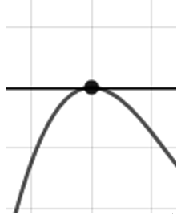
\includegraphics[width = 0.3\textwidth]{../Figures/polyZeroBehaviorCopyBA.png}\item 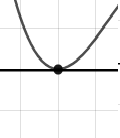
\includegraphics[width = 0.3\textwidth]{../Figures/polyZeroBehaviorCopyCA.png}\item 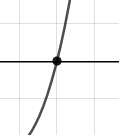
\includegraphics[width = 0.3\textwidth]{../Figures/polyZeroBehaviorCopyDA.png}\end{multicols}\item None of the above.
\end{enumerate} }
\end{enumerate}

\end{document}